%% DONE
\id{IRSTI 52.35.29}{https://doi.org/10.58805/kazutb.v.1.26-886}

\begin{articleheader}
\sectionwithauthors{Ye.S.Abdrakhmanov, Kh.B.Temirtas, B.T.Yermagambet, Zh.M.Kassenova, Zh.T.Dauletzhanova, M.K.Kazankapova, N.Sh.Akimbekov, K.T.Tastambek}{PRODUCTION OF HIGH-CALORIC COAL BRIQUETTES FROM THE EKIBASTUZ COAL DEPOSIT}

{\bfseries
\textsuperscript{1}Ye.S. Abdrakhmanov\alink{https://orcid.org/0000-0001-9726-1624},
\textsuperscript{1}Kh.B. Temirtas\alink{https://orcid.org/0000-0002-6580-2085},
\textsuperscript{2,3}B.T. Yermagambet\alink{https://orcid.org/0000-0003-1556-9526},
\textsuperscript{2,3}Zh.M. Kassenova\alink{https://orcid.org/0000-0002-9497-7319},
\textsuperscript{2,3}Zh.T. Dauletzhanova\textsuperscript{\envelope } \alink{https://orcid.org/0000-0002-9497-7319},
\textsuperscript{2,3}M.K. Kazankapova\alink{https://orcid.org/0000-0001-9016-3062},
\textsuperscript{4}N.Sh. Akimbekov\alink{https://orcid.org/0000-0002-5262-5155},
\textsuperscript{4}K.T. Tastambek\alink{https://orcid.org/0000-0002-2338-8816}}
\end{articleheader}

\begin{affiliation}
\emph{\textsuperscript{1}Toraighyrov university, Pavlodar, Kazakhstan,}

\emph{\textsuperscript{2}Institute of Coal Chemistry and Technolog» LLP, Astana, Kazakhstan,}

\emph{\textsuperscript{3} K.Kulazhanov named Kazakh University of Technology and Business, Astana, Kazakhstan,}

\emph{\textsuperscript{4}SRI «Sustainability of ecology and bioresources», KazNU named after al-Farabi, Almaty, Kazakhstan,}

\raggedright \textsuperscript{\envelope }{\em Corresponding-author: \href{mailto:kaliyeva_zhanna@mail.ru}{\nolinkurl{kaliyeva\_zhanna@mail.ru}}}
\end{affiliation}

The article provides information on the coal briquetting process, the
briquetting process, and establishes the mechanism of coal briquettes
structure formation taking into account the physicochemical and
structural-rheological properties of coal. Of great importance is the
uniform distribution of elementary size classes in the briquette charge.
It is achieved by choosing a coal classification process flow chart and
appropriate equipment. The coal size determines the total surface area
of the briquetting mass particles. The more developed this surface area
is, the greater the number of particle contacts inside the briquettes
and the more intense the action of molecular adhesion forces. The
increase in the total surface area of the grains can be achieved by
crushing. The main factors influencing the coal briquetting process are:
coal moisture and moisture distribution in individual classes, coal
size, distribution of elementary size classes in the briquette charge,
granulometric composition, pressure, pressing duration and temperature,
water content.

{\bfseries Keywords:} coal, ash content, briquetting, raw material quality
management, combustion heat, coal size.

\begin{articleheader}
{\bfseries ЕКІБАСТҰЗ КЕН ОРНЫНЫҢ КӨМІРІНЕН ЖОҒАРЫ КАЛОРИЯЛЫ КӨМІР БРИКЕТТЕРІН АЛУ}

{\bfseries
\textsuperscript{1}Е.С. Абдрахманов,
\textsuperscript{1}Х.Б. Теміртас,
\textsuperscript{2,3}Б.Т. Ермағамбет,
\textsuperscript{2,3}Ж.M. Касенова,
\textsuperscript{2,3}Ж.Т. Даулетжанова\textsuperscript{\envelope },
\textsuperscript{2,3}М.Қ. Қазанқапова,
\textsuperscript{4}Н.Ш. Акимбеков,
\textsuperscript{4}К.Т. Тастамбек}
\end{articleheader}

\begin{affiliation}
\emph{\textsuperscript{1}Торайғыров университеті, Павлодар, Қазақстан,}

\emph{\textsuperscript{2}«Көмір химиясы және технология институты» ЖШС, Астана, Қазақстан,}

\emph{\textsuperscript{3} Қ.Құлажанов атындағы Қазақ технология және бизнес университеті, Астана, Қазақстан,}

\emph{\textsuperscript{4} «Экология және биоресурстардың тұрақтылығы» ҒЗИ, әл-Фараби атындағы ҚазҰУ, Алматы, Қазақстан,}

\emph{e-mail: \href{mailto:kaliyeva_zhanna@mail.ru}{\nolinkurl{kaliyeva\_zhanna@mail.ru}}}
\end{affiliation}

Мақалада көмірді брикеттеу процесі, брикеттеу процесі туралы мәліметтер
келтірілген, көмірдің физикалық-химиялық және құрылымдық-реологиялық
қасиеттерін ескере отырып, көмір брикеттерінің құрылымдық түзілу
механизмі анықталған. Брикет шихтасындағы қарапайым кластардың біркелкі
таралуы маңызды. Оған көмірді жіктеудің технологиялық схемасын таңдау
және тиісті аппараттық дизайн арқылы қол жеткізіледі. Көмірдің мөлшері
брикеттелген масса бөлшектерінің жалпы бетін анықтайды. Бұл бет неғұрлым
дамыған болса, брикеттер ішіндегі бөлшектердің байланыс саны соғұрлым
көп болады және молекулалық байланыс күштерінің әсері күшейеді.
Дәндердің жалпы бетінің ұлғаюына ұсақтау арқылы қол жеткізуге болады.
Көмірді брикеттеу процесіне әсер ететін негізгі факторлар: көмірдің
ылғалдылығы және жекелеген кластардағы ылғалдың таралуы, көмірдің
үлкендігі, брикет шихтасындағы үлкендіктің қарапайым кластарының
таралуы, гранулометриялық құрамы, қысымы, престеу ұзақтығы мен
температурасы, судың мөлшері.

{\bfseries Түйін сөздер:} көмір, күл, брикеттеу, шикізат сапасын басқару,
жану жылуы, көмірдің мөлшері.

\begin{articleheader}
{\bfseries ПОЛУЧЕНИЕ ВЫСОКОКАЛОРИЙНЫХ УГОЛЬНЫХ БРИКЕТОВ ИЗ УГЛЯ ЭКИБАСТУЗСКОГО МЕСТОРОЖДЕНИЯ}

{\bfseries
\textsuperscript{1}Е.С. Абдрахманов,
\textsuperscript{1}Х.Б. Теміртас,
\textsuperscript{2,3}Б.Т. Ермагамбет,
\textsuperscript{2,3}Ж.M. Касенова,
\textsuperscript{2,3}Ж.Т. Даулетжанова\textsuperscript{\envelope },
\textsuperscript{2,3}М.К. Казанкапова,
\textsuperscript{4}Н.Ш. Акимбеков,
\textsuperscript{4}К.Т. Тастамбек}
\end{articleheader}

\begin{affiliation}
\emph{\textsuperscript{1}Торайгыров Университет, Павлодар, Казахстан,}

\emph{\textsuperscript{2}ТОО «Институт химии угля и технологии», Астана, Казахстан,}

\emph{\textsuperscript{3}Казахский университет технологии и бизнеса им.К.Кулажанова, Астана, Казахстан,}

\emph{\textsuperscript{4}НИИ «Устойчивости экологии и биоресурсов», КазНУ им. аль-Фараби, г. Алматы, Казахстан,}

\emph{e-mail: \href{mailto:kaliyeva_zhanna@mail.ru}{\nolinkurl{kaliyeva\_zhanna@mail.ru}}}
\end{affiliation}

В статье приведены сведения о процессе брикетирования угля, процесса
брикетирования, установлен механизм структурообразования угольных
брикетов с учетом физико-химических и структурно-реологических свойств
угля. Важное значение имеет равномерное распределение элементарных
классов крупности в брикетной шихте. Оно достигается выбором
технологической схемы классификации угля и соответствующим аппаратурным
оформлением. Крупность угля определяет суммарную поверхность частиц
брикетируемой массы. Чем более развита эта поверхность, тем больше число
контактов частиц внутри брикетов и интенсивней действие молекулярных сил
сцепления. Увеличение суммарной поверхности зерен может быть достигнуто
дроблением. Основными факторами, влияющими на процесс брикетирования
углей, являются: влажность угля и распределение влаги в отдельных
классах, крупность угля, распределение элементарных классов крупности в
брикетной шихте, гранулометрический состав, давление, продолжительность
и температура прессования, содержание воды.

{\bfseries Ключевые слова:} уголь, зольность, брикетирование, управление
качеством сырья, теплота сгорания, крупность угля.

\begin{multicols}{2}
{\bfseries Introduction.} Coal briquetting is the process of converting
fine fractions and coal dust into durable, compact briquettes that are
convenient for transportation, storage and use. This method not only
allows for the rational use of coal waste, but also improves its
calorific properties, reducing dust formation during combustion.
{[}1-2{]}.

The briquetting process includes several key stages:

- preparation of raw materials - coal is crushed to the required
fraction and, if necessary, dried to achieve the optimal moisture level;

- mixing with binders - to increase the strength and integrity of the
briquettes, binders such as petroleum bitumen, lignosulfonates,
molasses, liquid glass or cement are added to the coal mass6 The choice
of binder depends on the type of coal and the requirements for the final
product;

- forming briquette - the prepared mixture is fed into a press, where
briquettes of a given shape and size are formed under high pressure;

- drying and cooling - after pressing, the briquettes are dried to
remove excess moisture and increase strength, and then cooled to room
temperature {[}3-5{]}.

This method provides more efficient use of coal raw materials and
reduces the negative impact on the environment. Figure 1 shows
briquetted coal.

To organize the briquetting process, specialized production lines are
used, which include:

- crushers - designed to crush coal to a given fraction.

- mixers - ensure uniform distribution of binders in the coal mass.

- briquette presses - form briquettes under high pressure, giving them
the required density and shape.

- drying units - remove excess moisture, increasing the strength and
stability of the finished briquettes.

The combination of these elements allows for high process efficiency and
a high-quality final product {[}6-9{]}. Coal briquetting plants are
shown in Figure 2.

The advantages of coal briquettes are:

- high calorific value: briquetted coal has a calorific value of at
least 6000 kcal/kg;

- ease of transportation and storage: briquettes have a uniform shape
and density, which facilitates their transportation and storage.

- environmental friendliness: when burning, high-quality briquettes emit
less smoke and harmful gases, burn out completely, leaving a minimum amount of ash.
\end{multicols}

\begin{figure}[H]
	\centering
	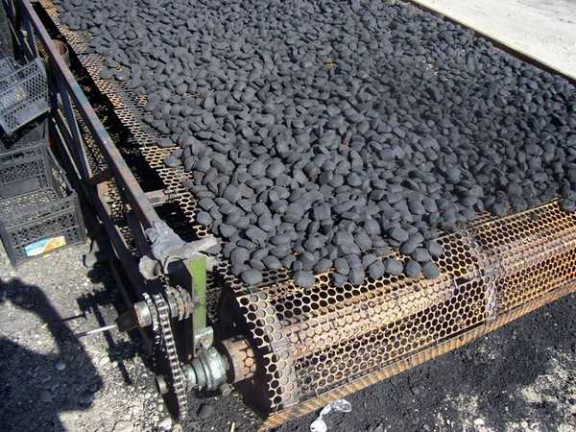
\includegraphics[width=0.6\textwidth]{media/gorn2/image2}
	\caption*{Fig. 1 - Briquetted coal}
\end{figure}

\begin{figure}[H]
  \centering
  \begin{subfigure}{0.45\textwidth}
    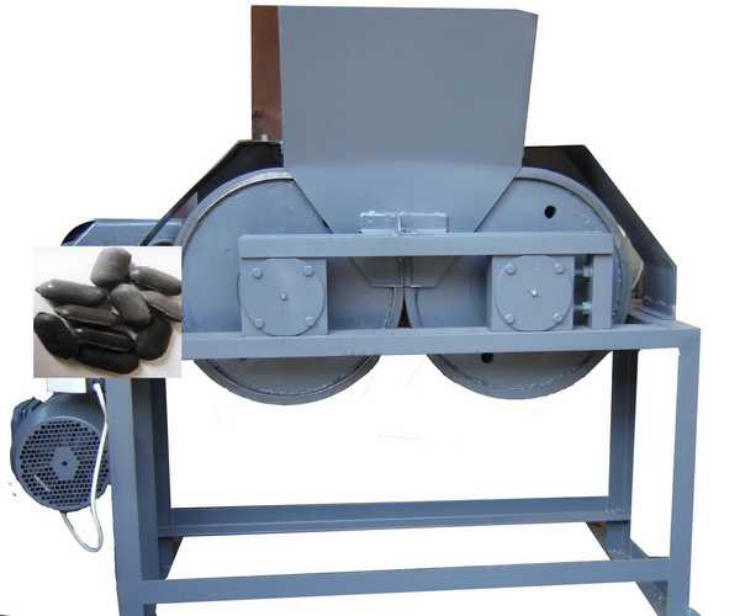
\includegraphics[width=\textwidth]{media/gorn2/image3}
  \end{subfigure}%
  ~%
  \begin{subfigure}{0.45\textwidth}
    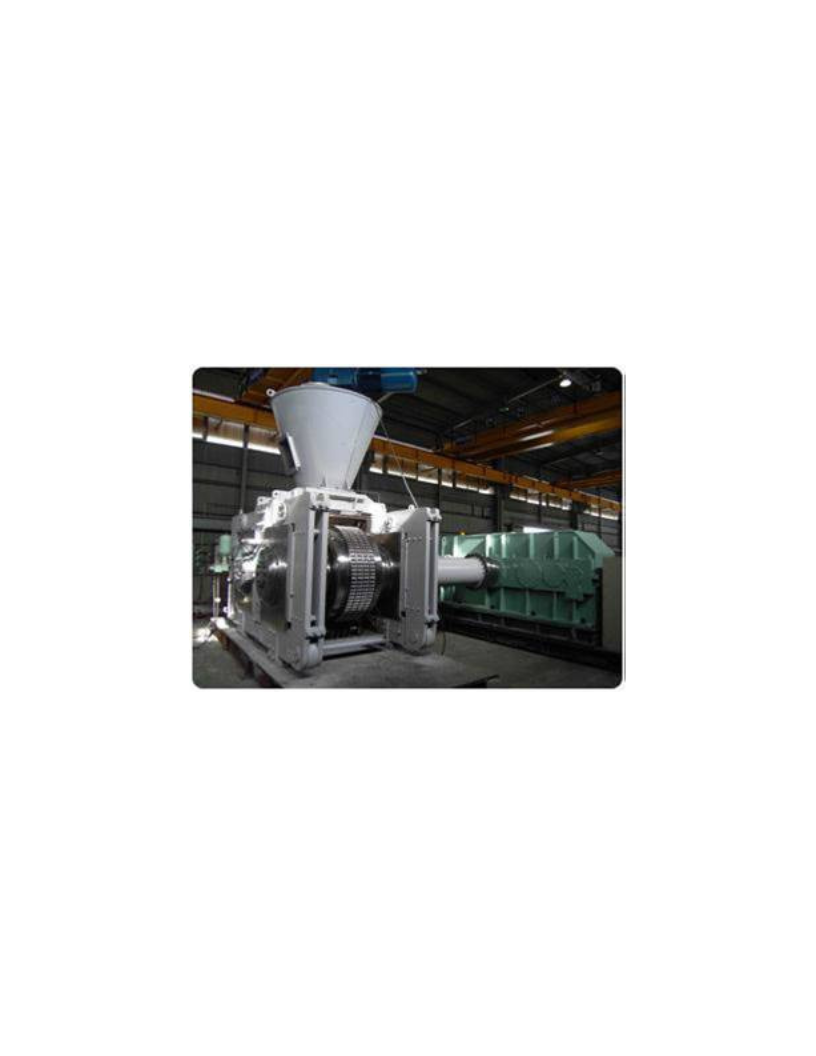
\includegraphics[width=\textwidth]{media/gorn2/image4}
  \end{subfigure}
  \caption*{Fig. 2 - Coal briquetting plants}
\end{figure}

\begin{multicols}{2}
In the work {[}10{]} within the framework of the work performed on the
use of coal enrichment waste, their experimental combustion was carried
out, technologies for granulation and further use were developed. For
the preparation of granules, the following are used: coal enrichment
waste, marble chips for binding sulfur oxides, and for the formation of
granules in order to prevent "smearing" of dust preparation equipment,
bitumen emulsion is added.

In the work {[}11{]} modern technologies for obtaining coal-water fuel
from coal enrichment waste are considered and are being developed mainly
in three directions: using wet grinding vibratory mills, using
cavitation devices, hydraulic shock technologies based on disintegrators
and rotary pulse devices.

The work {[}12{]} presents studies that the company OJSC Irkutskenergo
is currently developing in the areas of using waste from enriching
Cheremkhovo coals. One of the promising areas is the preparation and
combustion of water-coal fuel.

In the work {[}13{]} a computer modeling of coal combustion technology
in an oxygen-enriched environment is presented. Determination of the
degree of burnout, volatile substances and NO formation. A computer
model CFD (Computational Fluid Dynamic) of oxy-coal combustion
technology has been developed to study the process of coal combustion in
an oxygen-enriched environment.

The work {[}14{]} shows the development of the structure of a
vacuum-technological line for the production of environmentally
friendly, energy-efficient fuel obtained from raw materials of organic
origin, in particular, peat and coal.

A review of the work shows that insufficient attention has been paid to
issues of involving substandard coal fines in production, including
through enrichment and briquetting, which demonstrates the relevance of
this area.

{\bfseries Materials and Methods.} The coals of the Ekibastuz basin were
selected for the study. Six coal seams of working capacity have been
identified in the Ekibastuz basin, of which seams 6 and 5 are confined
to the Ashlyarik suite, and the rest are confined to the Ekibastuz. The
seams of the Ekibastuz suite are industrial and under development. The
coals of the basin are hard, humus, highly mineralized, and are
characterized by a complex substance-mineralogical composition. The ash
content of the coals is very high and reaches 40-49\%.

The Ekibastuz coal basin is developed by an open-pit method, which in
turn has a negative impact on the environmental situation in the region.
Polluting factors here are stripping operations and waste dumps after
them. One of the most severe polluting factors is the wind blowing of
coal dust and fines from open-pit coal mines and waste dumps. The
essence of the idea is to obtain briquettes from fine coal and dust of
high-ash coals of the Ekibastuz deposit with the possibility of
subsequent coking by increasing the carbon content, i.e. the calorific
value. One of the problems of briquetting at the moment is the
impossibility of obtaining briquettes without adding non-combustible
binders, which, in turn, will again increase the already high ash
content of the briquettes. As a solution, the possibility of obtaining
processed organic waste products of cattle or some by-products of oil
distillation as a binder, which are combustible substances and will not
reduce the percentage of the calorific value of the briquette, is being
considered.

Coals can be considered as a specific hydrated amorphous polymer of
irregular structure. Its properties are largely determined by colloidal
swelling processes. Briquetting of such substances should be presented
as a complex multi-stage process of forming a strong autohesive complex
due to high pressing pressures. There are several hypotheses about the
mechanism of coal briquettes formation.

Colloid hypothesis. According to this hypothesis, the briquetting of
coals is estimated from the position of molecular forces. The basis is
the mechanism of interaction between coal particles in the presence of
water and without it. According to this hypothesis, the formation of
briquettes is explained by the action of cohesive forces.

Bitumen hypothesis. According to the bitumen hypothesis, coal
briquetting is presented as a process similar to briquetting of minerals
with a binder. It is believed that the role of binders is played by
bitumens contained in coals. Coal bitumens are products of the
decomposition of resins, waxes and fatty acids. They consist of a
mixture of hydrocarbons, alcohols, acids and ethers. The bitumen content
in young coals is 10--20\%. Bitumens melt at a temperature close to 90
°C. In the molten state, bitumens have good adhesive properties. When
cooled, they solidify and acquire a fairly high strength.

The total surface area (cm\textsuperscript{2}) of crushed grains in one
briquette can be calculated as follows:

\begin{equation}
S_v = Sa,
\end{equation}

where S - surface of particles obtained from crushing one grain,
cm\textsuperscript{2}; \emph{а} - number of grains in a briquette.

\begin{equation}
    S = \frac{\pi D^3}{d}
\end{equation}

where {\bfseries D} -- average grain size before crushing, cm;

\emph{d} -- average grain size after crushing, cm.

\begin{equation}
    a = \frac{6M}{\pi D^3 \gamma}
\end{equation}

where \emph{М} -- briquette weight, g;

\emph{γ} -- bulk density of briquette, g/cm\textsuperscript{3}.

Substituting the corresponding values \hspace{0pt}\hspace{0pt}of S and
\emph{а} into formula (1), we obtain

\begin{equation}
    S_v = \frac{6M}{d\gamma}
\end{equation}

{\bfseries Results and Discussion.} Of great importance is the uniform
distribution of elementary size classes in the briquette charge. It is
achieved by choosing a technological scheme for coal classification and
the corresponding equipment design. Briquettes have maximum strength
with the following ratio of classes of the briquetting mixture: 0--1 mm
about 50\%, 1--2 mm -- 40--45\% and 2--4 mm --5--10\%. Dust particles
(less than 0.2 mm) have a negative effect on briquetting. Their content
should not exceed 8--10\%.

The size of the coal determines the total surface area of
\hspace{0pt}\hspace{0pt}the particles of the briquetted mass. The more
developed this surface area is, the greater the number of particle
contacts inside the briquettes and the more intense the action of
molecular adhesion forces. The increase in the total surface area of
\hspace{0pt}\hspace{0pt}the grains can be achieved by crushing.
Briquettes made of fine coal have fewer internal defects, a higher
packing density, and better plasticity of the briquetted mass. Hence, a
more uniform distribution of pressure throughout the entire volume of
the briquettes. The optimal size, which ensures sufficiently high
strength of the briquettes, is within 0--2 mm. The technological scheme
of coal briquettes production is shown in Figure 3.
\end{multicols}

\begin{figure}[H]
	\centering
	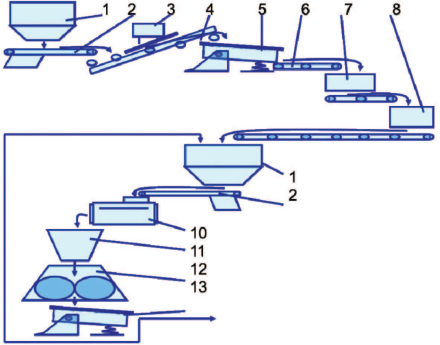
\includegraphics[width=0.6\textwidth]{media/gorn2/image5}
	\caption*{\normalfont\emph{1 - receiving bin, 2 - electrovibration feeder, 3 - lifting
magnet, 4 - belt conveyor, 5 -- screen, 6 - belt conveyor, 7 - roller
crusher, 8 - hammer crusher, 9 - belt conveyor, 10 -- mixer, 11 - hopper
with screw feeder, 12 - roller press, 13 - screen}}
	\caption*{Fig. 3 - Flow chart of coal briquettes production}
\end{figure}

\begin{multicols}{2}
The quality of briquettes is significantly affected by the distribution
of moisture in individual classes. Small particles of coal give up their
moisture faster and easier during drying than larger grains. Therefore,
to achieve high strength of briquettes, it is necessary to ensure a
minimum moisture difference between small and large grains. The moisture
difference is affected by the speed and method of drying the coal, the
difference in the sizes of the largest and smallest particles of the
material, and the nature of the coal. It is important to take into
account the uneven distribution of moisture in large grains. After
drying, moisture evaporates only from the surface, lingering in the deep
areas.
\end{multicols}

\begin{figure}[H]
	\centering
	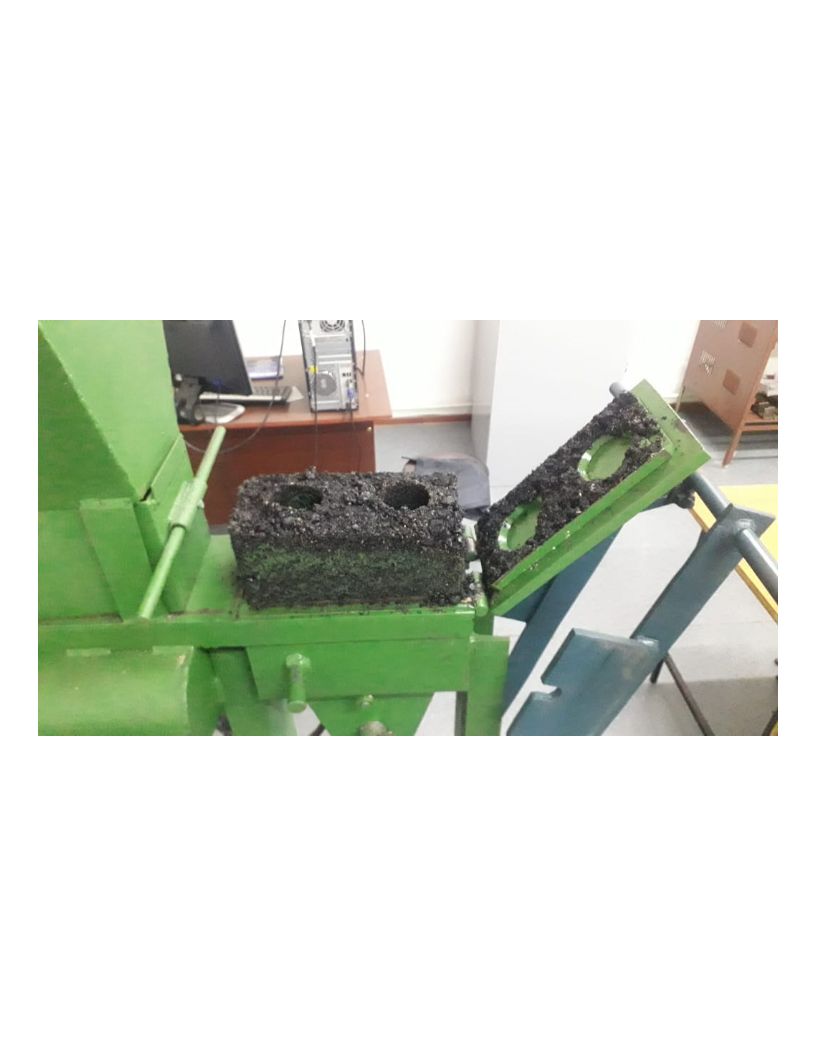
\includegraphics[width=0.8\textwidth]{media/gorn2/image6}
	\caption*{Fig. 4 - Sample of a briquette obtained in a semi-industrial plant}
\end{figure}

\begin{figure}[H]
  \centering
  \begin{subfigure}{0.45\textwidth}
    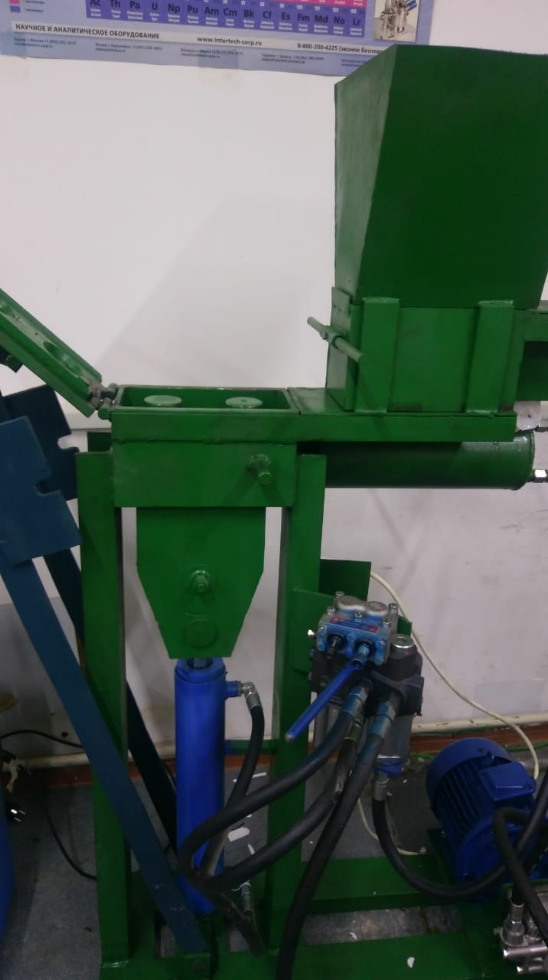
\includegraphics[width=\textwidth]{media/gorn2/image7}
  \end{subfigure}%
  ~%
  \begin{subfigure}{0.45\textwidth}
    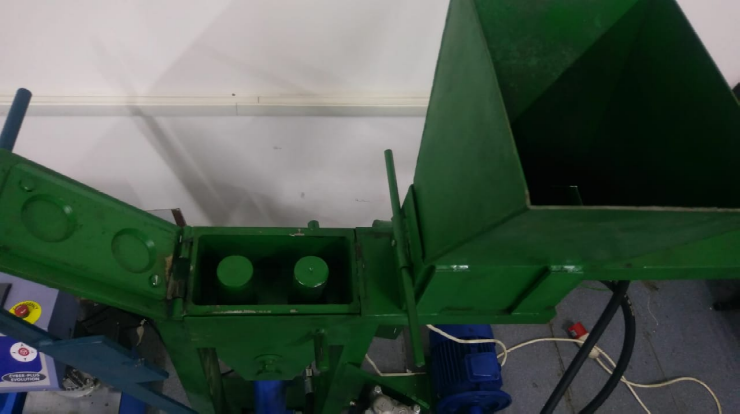
\includegraphics[width=\textwidth]{media/gorn2/image8}
  \end{subfigure}
  \caption*{Fig. 5 - Pilot plant for briquette production}
\end{figure}

\begin{multicols}{2}
The pressing factor is the most important for obtaining strong
briquettes. When pressing, under the action of mechanical pressure,
brown coal is compressed all around to form a lump product - a
briquette. The briquetted material (dry coal) can be considered as a
three-phase system: solid, liquid and gas. The gaseous phase is the air
in the pores of the coal and the spaces between individual grains. The
bulk of the air is easily removed during the pressing process. Only a
small amount of it remains in the pressed coal, weakening the structure
of the briquette. Therefore, during the pressing process, maximum air
removal is necessary through the appropriate gaps of the pressing
devices. A sample of a briquette obtained in a semi-industrial plant is
shown in Figure 4.

Before pressure is applied, coal particles contact each other at
individual points. With the application of pressure, point contacts
become weak surface contacts, and at maximum pressing force, they become
strong bonds of molecular adhesion forces. As pressure increases, the
entire mass of coal being briquetted is sequentially drawn into the
contact zone. The formation of the briquettes'{}
structure is accompanied by deformation of the coal in the press channel
and after the briquettes exit it. The deformation of the first period is
irreversible or residual, and of the second period it is reversible or
elastic.

The technology for producing briquettes can be based on waste from coal
enterprises, wood sawdust, lignin, and other industrial waste. Classic
pressing technology is used in preparing briquettes. The developed
process includes the stages of preliminary preparation of the initial
components, mixing and transferring polymers into a plastic state, and
molding briquettes using the viscous flow of the mass into molding
strains. The pilot plant for producing briquettes is shown in Figure 5.

Experiments were conducted to determine the physical and technical
characteristics of the briquettes depending on the conditions of their
preparation.

Table 1 shows that the amount of binder plays an important role in the
formation of the strength of the briquettes, which increases as the
binder increases. If we compare the strength of the briquettes with and
without a binder, we see that regardless of the drying temperature, the
strength of the briquettes increases by 1.5 times with the introduction
of a binder into the briquette.
\end{multicols}

\begin{table}[H]
\caption*{Table 1 - Physicochemical properties of the briquette depending on the input factors}
\centering
\begin{tblr}{
  width = \linewidth,
  colspec = {Q[83]Q[181]Q[146]Q[169]Q[135]Q[112]Q[108]},
  cells = {c},
  hlines,
  vlines,
}
Samples & Drying temperature, °C & Mass of binder, \% & Calorific value, MJ/kg & Ash content, ~\% & Humidity, ~\% & Durability, \% \\
1       & 25                     & -                  & 30,6                   & 1,9              & 14,2          & 32,2           \\
2       & 25                     & 5                  & 28,2                   & 3,4              & 15,3          & 54,1           \\
3       & 60                     & -                  & 28,5                   & 2,3              & 10,2          & 34,5           \\
4       & 60                     & 5                  & 27,8                   & 3,1              & 11,4          & 52,8           \\
5       & 60                     & 10                 & 27,3                   & 4,1              & 12,8          & 60,1           \\
6       & 100                    & -                  & 29,1                   & 3,1              & 8,3           & 23,4           \\
7       & 100                    & 5                  & 27,5                   & 2,1              & 9,5           & 45,7           \\
8       & 100                    & 10                 & 27,3                   & 2,6              & 11,2          & 64,7           
\end{tblr}
\end{table}

\begin{multicols}{2}
It is evident from Table 1 that the binder level has a significant
effect on all combustion properties studied. Increasing the binder level
decreases the calorific value. This is expected due to the decrease in
the proportion of semi-coke, which significantly contributes to the
overall calorific value of the mixture. It is also observed that the ash
content increases at drying temperatures from 25 to 600 °C, then
decreases at drying at 1000 °C, indicating that the lignosulfonate has
inorganic volatiles that are not combustible.

In an attempt to characterize the interactions occurring between the
lignosulfonate binder and the fine coal particles, we can assume the
following interaction mechanism. As preliminary observations show,
direct interactions between coal particles and lignosulfonate particles
in the granule are not observed with simple mechanical mixing, but
interactions occur through the surfactants of the lignosulfonate and the
coal surface.

Larger particles in the coal lead to adhesion between adjacent
particles. In addition, the presence of moisture enhances the activity
of surfactants. Lignosulfonates can act as a surfactant molecules with
spherical structures (micelles), where sulfonic acid and carboxylic acid
groups are located mainly on the surface of the hydrophobic hydrocarbon
core. These functional groups are available for interaction, especially
in the presence of surface moisture.

Study of adhesive-cohesive properties of petroleum pitch as a binder

Coal, enrichment and binding fractions enter the mixer from the
dispenser in strictly calculated proportions. The purpose of mixing this
batch is to maximize their averaging among themselves and to envelop the
surfaces of coal and enrichment particles with a thin molten film of
petroleum pitch (binder).

Mixing of briquette masses is the first stage of manifestation of
adhesive interaction of components and homogenization of the system. The
entire complex of adhesive phenomena is the result of manifestation of
molecular interaction: from weak van der Waals forces to hydrogen bonds
of chemical nature. To calculate the theoretical bond strength for any
molecular forces Fm, one can use the transformed Morse equation {[}15,
16{]}:

\[Fm = \frac{bD}{2}\]

where b -- constant associated with the magnitude of the amplitude of
oscillation of interacting particles;

\emph{D} -- bond dissociation energy.

The formation of a particular type of bond is determined by its
activation energy. Low activation energy is characteristic of molecular
adhesion, which is carried out under the influence of Van der Waals
forces, as well as adhesion due to the formation of hydrogen bonds
through functional groups located on the surface of particles and in the
binding groups.

The most important thermodynamic characteristic of adhesion in the
briquette composition is the wettability of the substrate by the
adhesive and the surface tension at the phase boundary. The particles of
coal and enrichment remain permanently solid during the mixing process,
so for the sake of convenience we will call them the base.

In contrast, petroleum pitch, being initially a powder composite, will
become a liquid wetting binder during the mixing process under the
influence of externally introduced temperature into the working cavity
of the mixer. Therefore, petroleum pitch is further called the binder.

The work of wetting the solid surface of the base (substrate) by the
binder can be expressed by the Dupre equation

\begin{equation*}
    W_a = \sigma_{tg} + \sigma_{jg} - \sigma_{tj}
\end{equation*}

where W\textsubscript{a} -- reversible work, Н/m;

σ\textsubscript{tg}, σ\textsubscript{jg}, σ\textsubscript{tj} -- surface
tension at the liquid-gas interface, Н/m.

The equilibrium condition for drops of a binder on a solid surface,
expressing Young' s equality

\begin{equation*}
    \delta_{\text{tg}} = \delta_{\text{tj}} + \delta_{jg} \cos\varphi
\end{equation*}

The present equation with the Dupre equation can be transformed into the
Dupre-Young equality.

\begin{equation*}
    W_a = \sigma_{\text{jg}} (1 - \cos\varphi)
\end{equation*}

where φ -- contact angle.

From the Young equation we can derive

\begin{equation*}
    \cos\varphi = \frac{\sigma_{tg} - \sigma_{tj}}{\sigma_{jg}}
\end{equation*}

In order to achieve comparability in the assessment of adhesive
activity, several bases must meet the conditions σ\textsubscript{jg} =
соnst, then \emph{Wa = f(соsφ).}

In this case, the adhesion work will be a function of one variable --
the contact angle. This is achieved by using the same adhesive for all
base samples, i.e. the same binder (petroleum pitch).

For the adhesion to be high enough, the condition must be met:

\begin{equation*}
    \sigma_{\text{tg}} > \sigma_{\text{jg}} + \sigma_{\text{tj}}
\end{equation*}

When wetting the base surface with a binder \(соs\varphi > 0\), and
\emph{φ \textless{} 900}, in the absence of wetting φ \textgreater{}
900.

Adhesive interaction phenomena can be attributed to relatively
low-temperature processes. The bonds formed in this case are
characterized by low interaction energy: 4.2 kJ/mol for Van der Waals
forces, 21 ÷ 42 kJ/mol for hydrogen bonds. At the same time, the
formation of chemical bonds in the so-called adhesive-substrate
"cross-linking" reactions have an interaction energy 15 ÷ 20 times
higher and are possible in the process of compaction of the hot
briquette mass. Only this type of reaction leads to the formation of the
composite structure.

However, the structure of the contact layer is generated in the process
of adhesive interaction, the compaction process (pressing) only
completes the previously formed system. The presence of various adhesion
defects (unfilled pores, unwetted areas, cracks, air inclusions, etc.)
are potential sources of local stress and destruction of the briquette
structure.

Maximum enveloping (wetting) of the base with a binder is the most
important task of mixing. Of course, the most favorable course of this
process would be the spontaneous entry of the binder into the pores of
the base particles. The depth h of spontaneous penetration of the liquid
phase into the pores under the action of capillary forces (at a contact
angle of wetting φ \textless{} 900) is determined by the equation:

\begin{equation*}
    h = \frac{2\sigma_{jg} \cos\varphi}{\rho r g}
\end{equation*}

where \emph{σ\textsubscript{jg}} -- surface tension of the binder Н/m;

\emph{r} -- pore radius, m;

\emph{g} -- acceleration of gravity, m/s\textsuperscript{2}.

Using the Poiseuille equation for a laminar flowing liquid of viscosity
μ, one can calculate the time τ required for the binder to pass into a
capillary of radius r to a depth h. The flow velocity of the liquid w is
equal to:

\begin{equation*}
    w = \frac{\Delta P_{k}}{h} \cdot \frac{r^2}{8\mu}
\end{equation*}

If \emph{τ = h/w} the value of capillary pressure from the Laplace
equation:


Calculations using these formulas show that the process of spontaneous
impregnation of the base with a binder is very long (up to 4 hours or
more). This process can be accelerated by almost an order of magnitude
when the contact angle is reduced from 800 to 100.

Pores up to 0.2 mm are completely filled with the binder due to
capillary forces (taking into account the maximum grain size of the base
of 1.2 mm). It should be taken into account, however, that in the case
of a dead-end pore (the mixture borders the walls of the molding
tooling), the action of the capillary forces will be inhibited due to
the counterpressure created in the pore itself. If in a pore of length
l\textsubscript{0} part of its length l is occupied by the binder, then
in the free part the air pressure will be

\[\mathrm{\Delta}Р^{1} = \frac{l_{0}}{l_{0} - l}\]

The condition of equilibrium of the capillary process will be equality

\[\mathrm{\Delta}Р^{1} = \mathrm{\Delta}{Р_{к}}\frac{l_{0}}{l_{0} - l} = \frac{2\sigma_{jg}соs\varphi}{r}\]

Where does the depth of penetration of the binder into the dead-end pore
under the action of capillary forces amount to

\[l = l_{0}\left( \frac{1 - r}{2\sigma_{jg}соs\varphi} \right)\]

That is, it is determined by the surface tension of the binder, the
wetting angle, the radius and length of the pores. It is obvious that
for maximum filling of the pores it is necessary

\[\left( \frac{1 - r}{2\sigma_{jg}соs\varphi} \right) \rightarrow 1 \vee \left( \frac{r}{2\sigma_{jg}соs\varphi} \right) \rightarrow 0\]

For pores, this condition is satisfied when φ → 0, σ\textsubscript{jg} →
max. In real mixers, these conditions are achieved by additional
pressure ΔP created by the screw turns or mixer blades. In this case,
the total pressure in the capillary will be

\begin{equation*}
    P = \Delta P_k + \Delta P
\end{equation*}

If the value of P is insufficient to squeeze air out of a dead-end pore,
it may remain unfilled even in the finished briquette. The nature of
filling a narrowing-expanding pore connected by a neck is somewhat
different. In the real structure of the base, this geometry of pores is
more common than pores of the correct geometric shape.
\end{multicols}

\begin{figure}[H]
    \centering
    \begin{subfigure}{0.45\textwidth}
        \centering
        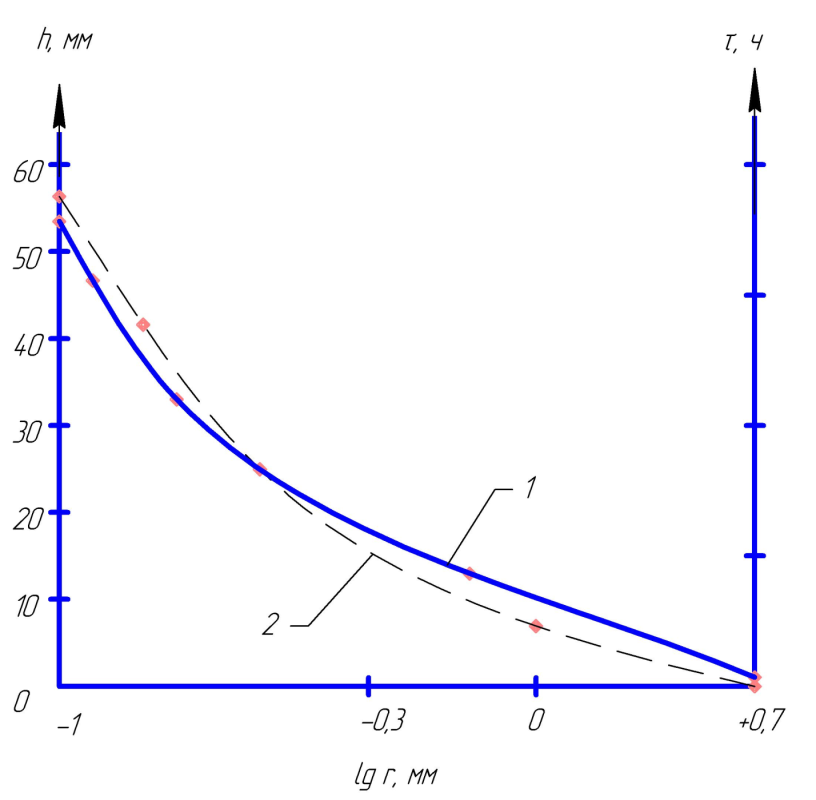
\includegraphics[width=\textwidth]{media/gorn2/image9}
        \caption*{Fig. 6 - Dependence of the height (row 1) and time (row 2) of the capillary rise of the binder on the pore diameter}
    \end{subfigure}
    ~
    \begin{subfigure}{0.45\textwidth}
        \centering
        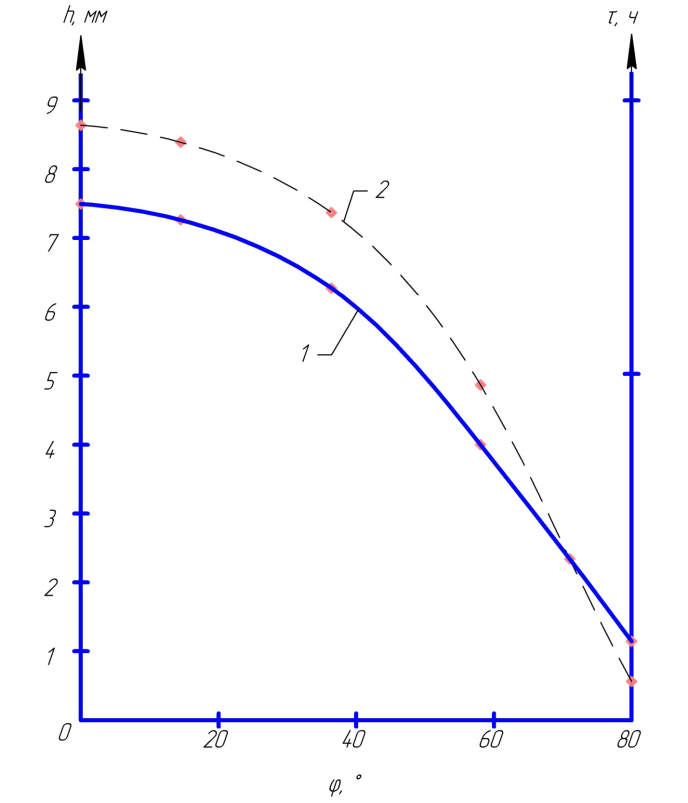
\includegraphics[width=\textwidth, height=\textwidth]{media/gorn2/image10}
        \caption*{Fig. 7 - Dependence of the height (1) and time (2) of the capillary rise of the binder on the wetting angle of the base by the binder}
    \end{subfigure}
\end{figure}

\begin{figure}[H]
	\centering
	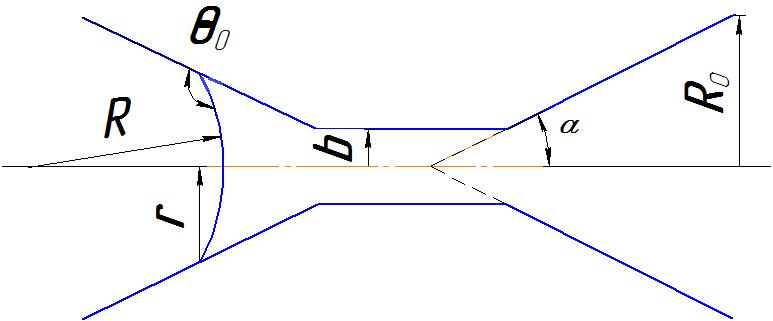
\includegraphics[width=0.6\textwidth]{media/gorn2/image11}
	\caption*{Figure 8 − Schematic of a narrowing - expanding pore}
\end{figure}

\begin{multicols}{2}
The pressure of the binder in this case is also determined by the
Laplace equation. In a narrowing drop, the radius of curvature of the
meniscus R, will be equal to

\begin{equation*}
    R = \frac{r}{\cos(\varphi + \alpha)}
\end{equation*}

In the expanding part, the angle α has a minus sign. Accordingly, the
capillary pressure in the converging (+α) and expanding (−α) parts will
be

\begin{equation*}
    \Delta P_k = \frac{2\sigma_{jg} \cos(\varphi \pm \alpha)}{r}
\end{equation*}

In the connecting neck

\begin{equation*}
    \Delta P_k = \frac{2\sigma_{jg} \cos\varphi}{r}
\end{equation*}

The mixing process takes place in a temperature range 140 ÷ 180
\textsuperscript{0}С, at the same time
\(\varphi \approx 90 \pm 10^{0}\). From the given equations it is easy
to establish that the greatest negative pressure preventing the
penetration of liquid into the pore is created when the conical part of
the narrowing pore passes into the neck. This pressure can be called the
"breakdown pressure". Exceeding it allows one to overcome the "narrow"
section beyond which the binder fills the pore. This condition is
achieved by creating additional pressure in the mixer itself or by
achieving the wetting condition, when \(\varphi \ll 90^{0} + \alpha.\)

The interaction of soot dust particles (enrichment agent) with the
liquid phase of the binder is also associated with capillary phenomena
in briquette compositions. Let there be a thin layer of wetting liquid
between two closely located solid soot particles.
\end{multicols}

\begin{figure}[H]
	\centering
	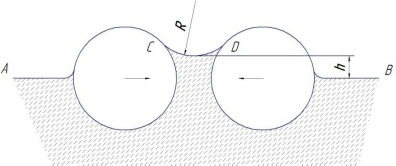
\includegraphics[width=0.6\textwidth]{media/gorn2/image12}
	\caption*{Fig. 9 - Movement of two particles on the surface of a liquid}
\end{figure}

\begin{multicols}{2}
The surface of the liquid, due to capillary phenomena, acquires a
concave shape, raised above the level AB to a height h. Then, according
to Laplace' s law, there will be a negative pressure
between the particles in the liquid, equal to

\begin{equation*}
    P = \frac{-2\sigma_{jg} \cos\varphi}{r}
\end{equation*}

In this case, atmospheric pressure will act on the outer surfaces of the
particles, and below atmospheric pressure on the inner surfaces (below
CD), which will lead to the particles coming closer together. Thus, a
closed film of dust particles is formed on the surface of the liquid.
The smaller the diameter of the dust particles, the stronger the forces
holding them. The wetting ability of a drop of binder covered with a
film is extremely low, which inhibits the processes of capillary
penetration of the binder into the pores of the base particles. The
filler and binder have a mutual influence in the composition of the
briquette composition. By adsorbing on the surface of the filler
particles, the molecules of petroleum pitch increase the effective
diameter of the particles, which entails an increase in the volume
concentration of the filler. According to the Einstein formula for
diluted suspensions, with an apparent increase in the volume fraction C
of solid spherical particles, the viscosity μ increases according to the
formula

\[\mu = \mu_{0}(1 + 2,5C)\]

where μ\textsubscript{0} -- viscosity at С = 0.

For concentrated systems according to the Gutman formula

\[\mu = \mu_{0}(1 + 2,5C + {14,1C}^{2})\]

For very high concentrations the formula is recommended

\[\frac{\mu}{\mu_{0}} = 2,5(1 - \varepsilon C)\]

where \(\varepsilon\) − coefficient depending on the filler
concentration

Viscosity is associated with the phenomenon of filler sedimentation in
the liquid phase of the binder. The resistance force experienced by a
solid spherical particle of radius r when moving in a viscous liquid is
determined by Stokes'{} law

\[F = 6\pi r\mu w\]

The maximum speed of a small ball falling in a viscous liquid is found
using a well-known formula in physics, which follows from
Stokes'{} law:

\[w_{pr} = \frac{\frac{2}{9}r^{2}g\left( \rho^{1} - \rho \right)}{\mu}\]

where \(\rho^{1},\rho\) -- particle and liquid density.

Using this formula, we calculated the dependence of the settling rate of
coal particles, anode dust in petroleum pitch at 170 -- 200
\textsuperscript{0}С.
\end{multicols}

\begin{figure}[H]
	\centering
	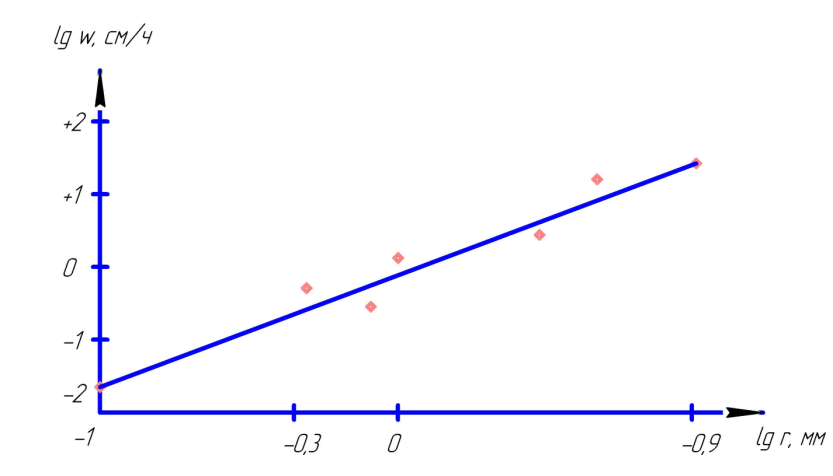
\includegraphics[width=0.6\textwidth]{media/gorn2/image13}
	\caption*{Fig. 10 - Dependence of the settling velocity of particles with a radius of 0.1 ÷ 8 mm in petroleum pitch}
\end{figure}

\begin{multicols}{2}
In the experiments, for greater clarity, a wider range of particle sizes
was taken from 0.2 to 16 mm, although in the briquette mass the
granulometry of coal is from 0.8 to 1.2 mm, and that of anode dust is
from 0.2 to 0.4 mm.

Thus, with an increase in the particle radius from 0.1 to 8 mm, the
settling rate increases from 0.024 to 118 cm/h. Let us further
recalculate the viscosity of the binder to the viscosity of the filled
system using the Gutman formula. Let us take the volume fraction of the
filler as 0.72, while the viscosity of the composition will be an order
of magnitude higher than the viscosity of the binder. Accordingly, the
settling rate will also decrease by an order of magnitude to 0.0024 ÷
11.8 cm/h.

The stability of the masses against sedimentation is a determining
factor for maintaining the specified recipe in the liquid phase of the
briquettes. The temperature dependence of viscosity, according to the
Frenkel-Eyring theory, is determined by the expression:

\[\mu = Ae^{\frac{\Delta G}{RT}}\]

where А -- constant;

G -- free energy of activation of viscous flow;

R -- gas constant.

This dependence is generally valid for the briquette mass. It is evident
from the equation that with an increase in temperature T, the viscosity
of the system decreases and with a large overheating, sedimentation can
reach significant values.

Based on the theoretical studies outlined above, we investigated the
adhesion processes in briquette compositions, namely, the adsorption of
petroleum pitch by the surface of a coal grain, the wetting of the coal
substrate with a drop of pitch, as well as the influence of various
factors on adhesion in the specified systems.

The dependence of the adsorption capacity of dispersed base powders on
their specific surface is shown in Figure 11, and on the grain size in
Figure 12.
\end{multicols}

\begin{figure}[H]
    \centering
    \begin{subfigure}{0.45\textwidth}
        \centering
        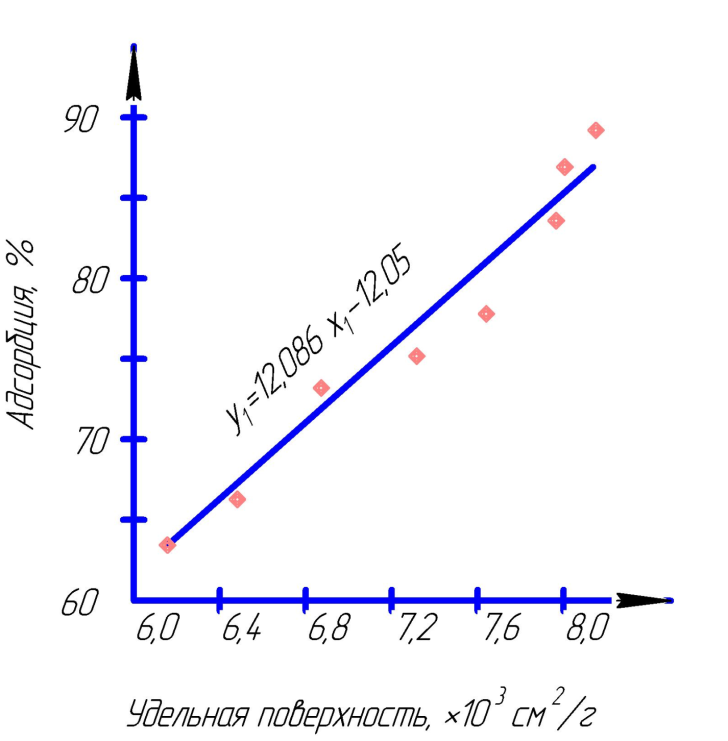
\includegraphics[width=\textwidth]{media/gorn2/image14}
        \caption*{Fig. 11 - Dependence of the adsorption capacity of powders on their specific surface area}
    \end{subfigure}
    ~
    \begin{subfigure}{0.45\textwidth}
        \centering
        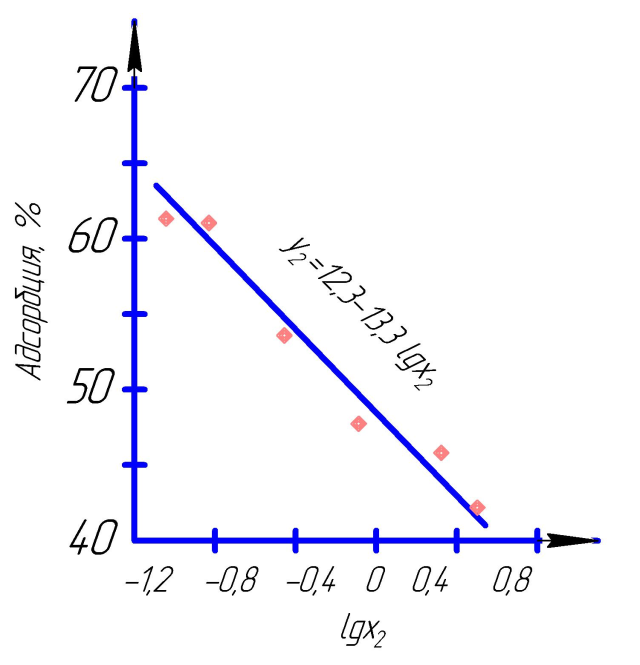
\includegraphics[width=\textwidth]{media/gorn2/image15}
        \caption*{Fig. 12 - Dependence of adsorption capacity of powders on particle size}
    \end{subfigure}
\end{figure}

\begin{multicols}{2}
Evaluation of the quality of mixing of briquette mass

Preparation of briquette mass consists of two closely related processes:
mixing (averaging) itself and physical and chemical processes of
interaction of all components of the briquette composition. These
processes are often superimposed on each other, and partially proceed
sequentially.

To evaluate the qualitative side of the mixing process, one of the
important indicators is the degree of homogenization of the mixed mass.
In the limit, a completely homogenized mass should have the same
component and grain composition in any macrovolumes. Therefore, the
measure for evaluating the mixer' s operation is the
standard deviation of the sample composition taken after a certain
mixing time, or the degree of mixing, expressing the ratio of the actual
deviation of a particular component of the mixture to the theoretical
standard deviation of an ideally mixed mixture. The latter indicator, in
the limit equal to 1 (or 100\%), is more visual for evaluating the
characteristics of the mixer' s operation.

Consequently, the evaluation of the quality of mixing can be partially
carried out from the standpoint of statistical distribution parameters.
There are dozens of formulas for quantitatively evaluating the
distribution of mixed components in the final products. The coefficient
of heterogeneity (variation) has become widespread as a criterion for
the quality of mixing.

\begin{equation*}
    V_{c} = \frac{100S}{\overline{m}} = \frac{100}{\overline{m}} 
    \sqrt{\frac{\sum_{i = 1}^{n} \left( X_{i} - \overline{m} \right)^{2}}{n - 1}}, \%
\end{equation*}

where S -- standard deviation;

\(\overline{m}\) -- arithmetic mean content of the controlled component
in all samples;

n -- number of samples;

\(Х_{i} -\)the value of random variable X in the i-th experiment.

It is advisable to evaluate the quality of mixing of masses using some
control fraction of base particles (for example, 0.8--1.2 mm or 1--1.5
mm) in single samples \emph{Сi}:

\begin{equation*}
    V_{c} = \frac{100S}{\overline{C}} = \frac{100}{\overline{C}} 
    \sqrt{\frac{1}{n - 1} \sum_{i = 1}^{n} \left( \overline{C}_{i} - \overline{C} \right)^{2}}, \%
\end{equation*}

where \(\overline{С}\) -- arithmetic mean of the number of particles in
the samples studied, \%.

However, as was indicated at the beginning of this section, mechanical
mixing (homogenization) in itself does not yet mean obtaining a
briquette mass as a stable polycomposition. The second stage - adhesion
(wetting, sorption), capillary impregnation, etc. ensure the stable
formation of the finest layers at the abrasive-substrate boundary,
connected by the action of van der Waals, molecular and electrostatic
forces. The presence of such forces leads to the formation of a solid
volumetric structure. Only after the completion of these processes does
the briquette mass turn into a cohesive, loose, extremely concentrated
and structurally stabilized substance. It is the spatial structure of
molecular forces that gives the substance plasticity, viscosity and
stability of the composition.

For a normal (Newtonian) liquid, the movement of layers is caused by an
arbitrarily small force. In structured systems, as a result of the
presence of a sufficiently strong continuous structural network, it is
necessary to apply some force to destroy it. According to a number of
studies {[}17 -18{]} , the flow of such a system begins only from the
moment when the shear stress R exceeds a certain critical value Rk,
necessary for the destruction of the structure formed in this system.
Such a flow is called plastic, and Rk is the yield point.

In the briquette mass at operating temperatures, a viscous flow is more
typical, as in a normal Newtonian fluid. In the mass of the mixture, as
a result of a sharp increase in the concentration of the base, one
should expect a noticeable manifestation of elastic plastic properties
and the yield point, which is especially important when forming
briquettes in roller presses. This is what ensures the preservation of a
stable shape of the briquettes after they exit the mold cells.

Considering the complexity of the above processes, the technological
assessment of the quality of mixing sand-coal masses has a number of
features. It is very important to assess the completion of the main
processes during mixing: homogenization, adhesive interaction,
enveloping, impregnation, etc. The rheological characteristics of the
masses (viscous flow and plasticity, sedimentation in the liquid phase
of the binder, pressing characteristics, etc.) are also taken into
account.

A study of the adhesive-cohesive properties of petroleum pitch as a
binder showed that the process of mixing coal and enrichment fractions
with pitch plays a key role in the formation of the structure of the
briquette mass.

{\bfseries Conclusion.} As a result of the theoretical analysis of the
briquetting process, the mechanism of coal briquettes structure
formation was established taking into account the physicochemical and
structural-rheological properties of coal. The main factors influencing
the coal briquetting process are: coal moisture and moisture
distribution in individual classes, coal size, distribution of
elementary size classes in the briquette charge, granulometric
composition, pressure, duration and temperature of pressing, that is, in
general, the structural-rheological and physicochemical properties of
the solid phase, as well as the water content. The application of high
pressure during briquetting brings the particles closer together and
increases interparticle contact, which results in an attractive force
between adjacent particles through weak Van der Waals forces. During
this process, particle deformation causes smaller binder particles to
fill the voids in the original briquette mixture.
\end{multicols}

\begin{center}
{\bfseries References}
\end{center}

\begin{references}
1. Adylov CH.A. Ehkonomicheskie aspekty briketirovaniya uglei s
pomoshch' yu svyazuyushchikh
rastitel' nogo proiskhozhdeniya // Nauka. Obrazovanie.
Tekhnika. - 2017. - No. 1. - P. 14-18. {[}In Russian{]}

2. Ismanzhanov A.I., Dzholdosheva T.Dzh., Adylov CH.A. Optimizatsiya
tekhnologii briketirovaniya uglei s produktami pererabotki biomassy
metodom matematicheskogo planirovaniya ehksperimenta // Nauka.
Obrazovanie. Tekhnika. - 2016. - No. 1. - P. 5-10. {[}In Russian{]}

3. Baiseitov M., Tulepov A., Zhapekova A. i dr. Sintez
ugol' nykh briketov v matritse polivinilkhlorida //
Promyshlennost'{} Kazakhstana. - 2020. - No. 1. - P.
34-36. {[}In Russian{]}

4. Baiseitov D., Tulepov M., Gabdrashova SH. i dr. Povyshenie
kaloriinosti i teplotvornoi sposobnosti ugol' nykh
briketov sostavov // Promyshlennost'{} Kazakhstana. -
2020. - No. 1. - P. 30-33. {[}In Russian{]}

5. Yusupov S.K., Ehshmetov I.D., Bekturdiev G.M. i dr. Modifitsirovannyi
svyazuyushchii dlya \\briketirovaniya uglya // Universum. - 2019. - No.
12. - P. 86-90. {[}In Russian{]}

6. Kuskov V.B., Skripchenko E.V., Kalashnikova V.YU. Razrabotka
tekhnologii polucheniya toplivnykh briketov iz malovostrebovannogo
uglerodsoderzhashchego syr' ya // Zapiski Gornogo
instituta. - 2012. - Vol. 196. - P. 147-149. {[}In Russian{]}

7. Drizhd N.A., Dauletzhanov A.ZH., Dauletzhanova ZH.T. i dr.
Issledovanie kachestva toplivnykh briketov iz
Shubarkol' skogo uglya // Gornyi zhurnal Kazakhstana. -
2021. - No. 9. - P. 44-49. {[}In Russian{]}

8. Loginov D.A., Chernykh A.P., Islamov S.R.
Ehksperimental' noe issledovanie vliyaniya davleniya na
protsess polukoksovaniya burogo uglya // Khimiya tverdogo topliva. -
2021. - No. 2. -P. 67-70. {[}In Russian{]}

9. Drizhd N.A., Dauletzhanova Zh.T., ,Zamaliyev N.M., Dauletzhanov A.Zh.
Influence of technological process parameters on qualitative
characteristics of coal thermolysis products // Naukovyi Visnyk\\
Natsionalnoho Hirnychoho Universytetu. -- 2021. -- No.1 P. 39-46
\href{https://doi.org/10.33271/nvngu/2021-1/039}{DOI
10.33271/nvngu/2021-1/039}

10. Abdrakhmanov Ye.S. Thermal capacity of enriched fuel briquets
produced from the fine of ekibastuz coal // Solid State Phenomena. --
2018 (Volume 284) P. 731-736
\href{https://doi.org/10.4028/www.scientific.net/SSP.284.731}{DOI\\
10.4028/www.scientific.net/SSP.284.731}

11. Fufaeva M.S., Manzhay V.N. Primenenie kriogelei dlya polucheniya
toplivnykh briketov iz \\melkodispersnykh uglerodsoderzhashchikh otkhodov
// Khimiya tverdogo topliva. - 2023. - No. 2-3. -P. 5-10.DOI
\href{https://doi.org/10.31857/S0023117723020032}{/10.31857/S0023117723020032}
{[}In Russian{]}

12. Buravchuk N.I., Guryanova O.V. Issledovanie vodostoikosti toplivnykh
briketov. - 2023. - No. 5. -P. 38-42
\href{https://doi.org/10.31857/S002311772305002X}{DOI
10.31857/S002311772305002X}{[}In Russian{]}

13. Аlvarez L., Gharebaghi M., Jones J.M., Pourkashanian M., Williams
A., Riaza J., Pevida C., Pis J.J., Rubiera F. CFD modeling of oxy-coal
combustion: Prediction of burnout, volatile and NO precursors release
{[}Text{]}: scientific publication / L. Alvarez {[}et al.{]} // Appl.
Energy. --Vol 104.-- 2013. -- P. 653--665
\href{https://doi.org/10.1016/j.apenergy.2012.11.058}{DOI
10.1016/j.apenergy.2012.11.058}

14. Ukhichev, A. S. Liniya ehnergeticheskogo obogashcheniya toplivnogo
syr' ya v vakuume: nauchnoe izdanie //
Nauchno-tekhnicheskaya konferentsiya s uchastiem zarubezhnykh
spetsialistov «Vakuumnaya nauka i tekhnikA». -- M., 2012. -- P. 62--63.
{[}In Russian{]}

15. Popov E.M. Issledovanie neftyanykh bitumov Ukrainy kak
svyazuyushchikh pri briketirovanii \\kamennogo uglya: dis. \ldots{} kand.
tekhn. nauk. -- Kiev: Institut uglekhimii NAN Ukrainy, 1958. -- 135 p.
{[}In Russian{]}

16. Ozhegov V.V. Briketirovanie poleznykh iskopaemykh. -- M.: Nedra,
2011. -- 304 p. {[}In Russian{]}

17. Ozerov A.V. Razrabotka tekhnologii briketirovaniya silikatnogo
flyusa i vybor ratsional' nogo \\svyazuyushchego dlya
briketirovaniya medno-nikelevogo kontsentrata: dis. \ldots{} kand.
tekhn. nauk. -Sankt-Peterburg: Sankt-Peterburgskii gornyi universitet,
2017. -- 152 p. {[}In Russian{]}

18. Abdrakhmanov, Y., Bogomolov, A., Bykov, P., Kuandikov, A. Thermal
capacity of enriched fuel briquets produced from the fine of ekibastus
coaL // International Journal of Engineering Technologies and Management
Research - 2017, No. 4(9), Р. 49--64.
\href{https://doi.org/10.29121/ijetmr.v4.i9.2017.99}{DOI
10.29121/ijetmr.v4.i9.2017.99}
\end{references}

\begin{authorinfo}
\emph{{\bfseries Information about the authors}}

Abdrakhmanov Ye.S. - Candidate of Technical Sciences, professor,
Toraighyrov university, Pavlodar, Kazakhstan, e-mail:
\href{mailto:erai1512@mail.ru}{\nolinkurl{erai1512@mail.ru}};

Temirtas Kh.B. - assistant, Toraighyrov university, Pavlodar,
Kazakhstan, e-mail:
\href{mailto:xamit1797@gmail.com}{\nolinkurl{xamit1797@gmail.com}};

Yermagambet B.T. - Doctor of Chemical Sciences, Professor, Academician
of KazNAEN, Project Manager, Chief Researcher, Director of LLP
"Institute of Coal Chemistry and Technology", Astana, Kazakhstan,
e-mail: \href{mailto:bake.yer@mail.ru}{\nolinkurl{bake.yer@mail.ru}};

Kassenova Zh.M. - Candidate of Chemical Sciences (PhD), Leading
Researcher, Deputy Director of LLP "Institute of Coal Chemistry and
Technology", Astana, Kazakhstan, e-mail:
\href{mailto:zhanar_k_68@mail.ru}{\nolinkurl{zhanar\_k\_68@mail.ru}};

Dauletzhanova Zh.T. - PhD, Associate Professor, Kazhach University of
Technology and Business, Astana, Kazakhstan, e-mail:
kaliyeva\_zhanna@mail.ru;

Kazankapova M.K. - PhD in Philosophy, Associate Professor, Corresponding
Member of KazNAEN, Leading Researcher, Head of Laboratory of LLP
"Institute of Coal Chemistry and Technology", Astana, Kazakhstan,
e-mail:
\href{mailto:maira_1986@mail.ru}{\nolinkurl{maira\_1986@mail.ru}};

Akimbekov N.S - PhD, Professor, Research Institute of ``Sustainability
of Ecology and Bioresources'', Almaty, Kazakhstan, e-mail:
\href{mailto:akimbeknur@gmail.com}{\nolinkurl{akimbeknur@gmail.com}};

Tastambek K.T.-- PhD, director, SRI Sustainability of ecology and
bioresources, Al-Farabi Kazakh National University,Almaty, Kazakhstan,
e-mail: kuanysh.tastambek@kaznu.edu.kz

\emph{{\bfseries Сведения об авторах}}

Абдрахманов Е.С. - к.т.н., профессор, Торайгыров Университет, Павлодар,
Казахстан. e-mail:
\href{mailto:erai1512@mail.ru}{\nolinkurl{erai1512@mail.ru}};

Теміртас Х.Б. -- ассистент, Торайгыров Университет, Павлодар, Казахстан.
e-mail:
\href{mailto:xamit1797@gmail.com}{\nolinkurl{xamit1797@gmail.com}};

Ермагамбет Б.Т. - доктор химических наук, профессор, академик КазНАЕН,
руководитель проекта, главный научный сотрудник, директор ТОО «Институт
химии и технологии угля», Астана, Казахстан, e-mail:
\href{mailto:bake.yer@mail.ru}{\nolinkurl{bake.yer@mail.ru}};

Касенова Ж.М. -- кандидат химических наук (PhD), ведущий научный
сотрудник, заместитель директора ТОО «Институт химии и технологии угля»,
Астана, Казахстан, e-mail:
\href{mailto:zhanar_k_68@mail.ru}{\nolinkurl{zhanar\_k\_68@mail.ru}};

Даулетжанова Ж.Т.- PhD, ассоциированный профессор,Казахский университет
технологии и бизнеса им.К.Кулажанова, Астана, Казахстан, e-mail:
\href{mailto:kaliyeva_zhanna@mail.ru}{\nolinkurl{kaliyeva\_zhanna@mail.ru}};

Казанкапова М.К.-PhD, ассоциированный профессор, чл.-корр. КазНАЕН,
ведущий научный сотрудник, заведующий лабораторией ТОО «Институт химии и
технологии угля», Астана, Казахстан, e-mail:
\href{mailto:maira_1986@mail.ru}{\nolinkurl{maira\_1986@mail.ru}};

Акимбеков Н.Ш. - PhD, профессор, НИИ «Устойчивости экологии и
биоресурсов», КазНУ им. аль-Фараби, Алматы, Казахстан, email:
\href{mailto:akimbeknur@gmail.com}{\nolinkurl{akimbeknur@gmail.com}};

Тастамбек К.Т. - PhD, директор НИИ «Устойчивости экологии и
биоресурсов», КазНУ им. аль-Фараби, Алматы, Казахстан, email:
\href{mailto:kuanysh.tastambek@kaznu.edu.kz}{\nolinkurl{kuanysh.tastambek@kaznu.edu.kz}}
\end{authorinfo}
